% main.tex

\documentclass[conference]{IEEEtran}
\IEEEoverridecommandlockouts
\usepackage{amsmath,amssymb,amsfonts}
\usepackage{algorithmic}
\usepackage{graphicx}
\usepackage{textcomp}
\usepackage{xcolor}
\usepackage{hyperref}
\usepackage[most]{tcolorbox}
\usepackage{graphicx}
\usepackage{svg}
\usepackage{booktabs}
\usepackage{soul} % for strikethrough \st
\usepackage[numbers,sort&compress]{natbib}
\usepackage{hyperref}
\usepackage{float}
\usepackage{multirow}

\graphicspath{ {./images/} }

% Define custom colors
% \definecolor{main}{HTML}{5989cf}
% \definecolor{sub}{HTML}{cde4ff}  
% Olive color palette
\definecolor{main}{HTML}{46AF70}
\definecolor{sub}{HTML}{E2F3E9}  
\definecolor{fontColor}{HTML}{2D5B9A}
\definecolor{white}{HTML}{FFFFFF}

% Yellow highlight
\newcommand{\hly}[1]{\sethlcolor{yellow}\hl{#1}}

% Research Question Box Style
\newtcolorbox{RQBox}{
    colback = sub!50, 
    colframe = main, 
    boxrule = 0pt, 
    leftrule = 6pt
}

% Glossary box style
\newtcolorbox{GlossaryBox}{
    enhanced,
    boxrule = 0pt,
    borderline = {0.75pt}{0pt}{main},
    borderline = {0.75pt}{2pt}{sub},
    colback = white
}


% Experiment Structure Rounded Box Style
\newtcolorbox{roundedBox}{
    fontupper=\footnotesize,
    colback=sub!30,
    boxrule=1.5pt,
    colframe=main,
    rounded corners,
    arc=5pt,
    boxsep=0pt, left=0pt, right=0pt,
}

% REST data example
\newtcolorbox{roundedBox-sm}{
    fontupper=\tiny,
    colback=sub!30,
    boxrule=0pt,
    colframe=main,
    rounded corners,
    arc=5pt,
    left=6pt, right=10pt,
}

\newtcblisting{databox}[1][]{%
  listing only,
  colback=gray!5,
  colframe=main!70!black,
  listing options={
    basicstyle=\ttfamily\tiny,
    breaklines=true,
    breakatwhitespace=true,
    columns=fullflexible
  },
  title=#1, % Accepts a custom title
  left=0mm, right=0mm, top=0mm, bottom=0mm,
  enhanced,
  sharp corners,
}

\def\BibTeX{{\rm B\kern-.05em{\sc i\kern-.025em b}\kern-.08em
    T\kern-.1667em\lower.7ex\hbox{E}\kern-.125emX}}
\begin{document}

\title{Evaluating Trade-offs of Quantized LLMs \\ for Requirements and Test Alignment}

% Evaluating Trade-offs of Using Quantized LLMs to Generate Trace Links Between Software Artifacts and Requirements In Software Projects That Utilize Traceability to Enhance Software Development --- A Comparative Experimental Empirical Investigative Analysis for the Purpose of Providing Insights

\author{
  \IEEEauthorblockN{Erik Lindstrand}
  \IEEEauthorblockA{\textit{Computer Science and Engineering} \\
  \textit{Chalmers and Gothenburg University}\\
  Gothenburg, Sweden \\
  elindstr@chalmers.se}
  \and
  \IEEEauthorblockN{Mariia Zabolotnia}
  \IEEEauthorblockA{\textit{Computer Science and Engineering} \\
  \textit{Chalmers and Gothenburg University}\\
  Gothenburg, Sweden \\
  mariiaz@chalmers.se}
  \and
  \IEEEauthorblockN{Michal Spano}
  \IEEEauthorblockA{\textit{Computer Science and Engineering} \\
  \textit{Chalmers and Gothenburg University}\\
  Gothenburg, Sweden \\
  spano@chalmers.se}
}

\maketitle

\begin{abstract}

Large Language Models (LLMs) have shown impressive capabilities in various domains due to their ability to process and interpret natural language. Meanwhile, as software systems continue to expand in size and complexity, the number of associated artifacts (e.g, Requirements and Test Cases) grows as well, leading to challenges in aligning REST (Requirement Engineering and System Test) efforts. There have been earlier initiatives in using LLMs for REST alignment, as it is a widely used measure for software quality assurance. However, the costs associated with model deployment and execution have limited their feasibility. There is a need for a faster yet reasonable solution to cope with the rate at which software artifacts keep growing.

In this paper, we investigate whether quantized LLMs can serve as a viable alternative, given their smaller size and less demanding hardware requirements. We choose Mistral, a widely used LLM, and evaluate it alongside three quantization techniques: AWQ, GPTQ, and AQLM, comparing all four Mistral versions with each other.
The experiment is performed with four requirement specification datasets encompassing more than 433 Requirements and 408 Tests in total.

We offer insights into the feasibility of adopting quantized LLMs for 
REST alignment, highlighting the efficacy, efficiency, and trade-offs of adopting such models, along with an actionable guidance for practitioners.

\end{abstract}

\begin{IEEEkeywords}
Large Language Models, REST, Traceability, Quantization, Software Testing
\end{IEEEkeywords}


\section{Introduction}\label{sec:intro}

The increasing complexity of modern software systems poses a variety of challenges. As software systems grow in size, so does the associated software and development artifacts. Managing these artifacts---and keeping them aligned with the software---becomes increasingly difficult as scale grows. To address this, researchers and practitioners have introduced \textbf{trace links} between artifacts as a way to manage the complexity \cite{jaber2013Effect}. 

Meanwhile, LLMs have proven to be exceptionally helpful in Software Engineering tasks \cite{naveed2024Comprehensive}; notably in requirements engineering \cite{arora2024Advancing} and software testing \cite{dakhel2024Effective, wang2024Software}. Their natural language understanding abilities have also been found to be useful for REST (Requirements Engineering and System Test) alignment efforts. Particularly, Ivarsson and Setterström have demonstrated that LLM-assisted trace link generation is feasible and yields satisfactory results \cite{ivarsson2023automated}. This idea is further supported by a study by Quinstedt and Lindgren who developed the \verb|REST-at| tool for automated requirements and tests alignment employing large language models \cite{quinstedt2024Optimizing}.

Although LLMs are showing potential as tools for REST alignment, previous research has demonstrated crucial challenges in their adoption\cite{quinstedt2024Optimizing}. Due to extensive hardware requirements, there is a need for a substantial up-front investment in order to run LLMs locally. In their study, Quinstedt and Lindgren observed that some models required up to 140 GB VRAM (Video RAM). Scalability is also a concern, leading to rapidly declining performance in terms of execution speed as input size increases. Because of these constraints, possible solutions include proprietary alternatives (e.g., OpenAI's ChatGPT, Google's Claude, etc.). However, these external solutions inherently come with additional security concerns \cite{quinstedt2024Optimizing}. These limitations make the practical application of LLMs for REST alignment more complicated and resource-demanding.

We select \textit{quantization} as a candidate solution to address the current obstacles hindering effective and affordable LLM-driven solutions for REST alignment \cite{bai2024beyond}. Quantization is a term used for a group of techniques that aim to reduce the memory usage of ML (Machine Learning) models for more effective resource utilization. Despite these benefits, a notable side effect of quantization is the associated loss of precision in the model's parameters, which may lead to a degradation in performance.

In this study, we investigate the trade-offs of utilizing quantized LLMs for REST trace-link generation. We consider metrics related to \textbf{efficacy}---measuring the quality of the produced results---and \textbf{efficiency}---measuring memory utilization and inference latency---in order to compare quantized models with their corresponding baseline model\footnote{In this paper, a ``baseline model'' refers to a non-quantized LLM version.}---in our case, different versions of Mistral.

\begin{RQBox}
    \textbf{RQ1}: How do quantized LLMs perform compared to non-quantized LLMs
    in terms of \textbf{efficacy} when used to create REST trace links?\\[0.5em]
    We evaluate model efficacy using the following metrics: \textit{balanced accuracy, precision, recall, F1-score}
\end{RQBox}

\begin{RQBox}
    \textbf{RQ2}: How do quantized LLMs perform compared to non-quantized LLMs in
    terms of \textbf{efficiency} when used to create REST trace links? \\[0.5em]
    We evaluate model efficiency using the following metrics: \textit{time-to-analyze, GPU memory usage (VRAM)}.
\end{RQBox}

\begin{RQBox}
    \textbf{RQ3}: What are the trade-offs of using quantized LLMs for REST alignment
    with respect to efficacy versus efficiency? \\[0.5em]
    We are particularly interested in investigating whether it is possible to balance acceptable recall and F1-score with lowered memory usage.
    % How does the artifact size affect the required compute time for RESST alignment?
    % In particular, we are interested in seeing the time-to-analyze metric over subset of 5, 10, 15, 25, 50, 75, 100 with the best performent model (as per RQ1, RQ2).
\end{RQBox}

Our findings arise from an experiment where we compare the generated trace links from each model against the \textit{ground truth}\footnote{The ground truth essentially stands for the desired mapping of requirements and tests, established by the respective company.} provided by our industry partner TestScouts\footnote{\url{https://testscouts.se/}}. We expand the existing \verb|REST-at| tool to support new quantized versions of existing baseline models. Afterwards, we execute the experiments on a cloud platform for scientific computing called \verb|Alvis|\footnote{\url{https://www.c3se.chalmers.se/about/Alvis}}. We access both baseline and quantized models from public repositories hosted on \textit{HuggingFace}\footnote{\url{https://huggingface.co/}}.


Our scientific contributions include: insights into the feasibility of utilizing quantized LLMs for REST alignment---in terms of efficacy and efficiency metrics; strategies for balancing trade-offs  when adopting quantized LLMs. We are also offering concrete guidelines for adopting quantization in industrial REST applications based on our findings. % + opening up questions for further research - is that a contribution?
Furthermore, our technical contributions include the expansion of the REST-at tool to support quantized models; we are also updating the tool to comply with other software updates that were introduced after it was developed and was affecting tool usability.


\section{Background \& Related Work}\label{background}

\subsection{Requirements Engineering and System Testing Alignment}

REST (Requirements Engineering and System Testing) alignment has been the subject of prior research studies, as has been shown in systematic literature mappings \cite{barmi2011Alignment, karhaapa2017What}. Achieving REST alignment involves activities that coordinate Requirements Engineering and System Testing efforts in order to optimize product development \cite{unterkalmsteiner2014Taxonomy}. Traceability is one of the tools that can be used to achieve alignment through the structuring of artifacts, such as requirement specifications and test cases, by creating connections (or traces) that help to evaluate and improve requirements coverage \cite{bjarnason2014Challenges}. Jaber et al. define a trace link as any link between different artifacts, such as a particular \textit{code element} (e.g., software test) in relation to a \textit{design element} (e.g., requirement specification) \cite{jaber2013Effect}. 

Real-world challenges in aligning RE and ST practices have been examined in previous case studies \cite{bjarnason2014Challenges,gomes2017Challenges}. According to both Bjarnason et al. and Gomes et al., introducing tracing between requirements and test cases is costly, meanwhile, a lack of traceability also comes with significant additional cost. There is also significant challenge in updating and maintaining traces between RE and ST artifacts, e.g., when requirements change. Moreover, the case study by Bjarnason et al. identifies a need, among the companies involved in the study, for tools that can manage REST traceability artifacts \cite{bjarnason2014Challenges}.

\subsection{Automated REST Alignment Using LLMs} 

There have been studies on the development of more advanced tools to aid in the trace creation process, with Ivarsson and Setterström showing promise in automating the process using LLMs by leveraging OpenAI’s GPT-3.5-turbo model\cite{ivarsson2023automated}. Their tool achieved an average of 86.394\% across accuracy and recall, although with limitations in terms of precision with an average of 45.582\%. Notably, the computational complexity is nonlinear in relation to the input size (requirements + test cases), resulting in an exponentially growing cost both financially and in \textit{time-to-analyze}, i.e., returning the results (trace links), which negatively impacts scalability \cite{ivarsson2023automated}. Furthermore, the study by Ivarsson and Setterström included identifying the main requirements for an automated REST tracing tool by performing literature reviews as well as conducting interviews with practitioners working at TestScouts, a company specializing in software testing \cite{ivarsson2023automated}.

Building on the work of Ivarsson and Setterström, Quinstedt and Lindgren conducted a study in which they evaluated and compared the efficiency of several different LLMs in creating REST trace links \cite{quinstedt2024Optimizing}. The requirements identified in Ivarsson and Setterström's study \cite{ivarsson2023automated} were further refined in collaboration with the same industry partner, TestScouts. These requirements were then used to develop a tool called \textit{REST-at} (REST alignment tool) which is capable of creating REST trace links by interfacing with proprietary models, such as OpenAI's GPT-4, through the use of APIs, in addition to using non-proprietary locally stored LLMs. Importantly, their study showed that smaller LLMs (in terms of number of parameters) were capable of achieving comparable results with much larger LLMs, with LLAMA 3 (70B parameters) achieving a 100\% recall score on the GBGE dataset, compared to GPT-3.5 (175B parameters) which had a recall score of 90.87\%.

However, Quinstedt and Lindgren's study also identified a key challenge in regards to hardware requirements and cost, due to the fact that running the LLMs require substantial computational resources. For instance, running the previously mentioned LLAMA 3 model with its 70B parameters requires 140 GB VRAM \cite{quinstedt2024Optimizing}. In order to mitigate this challenge, the study had to be adapted to instead run the models on the Alvis research cloud  infrastructure, offering significantly more computational power.

Given the challenges faced due to hardware constraints when utilizing LLMs, there is a need to explore techniques that would reduce the GPU memory usage. Moreover, it is still unclear whether using quantized models is useful for the purposes of REST alignment. Hence, we identify a gap in the current research regarding the application of quantized LLMs for the purpose of REST alignment. Thus, we explore LLM quantization methods as a viable technique to allow for models to run in a non-cloud environment while retaining reasonable performance in terms of automating REST traceability.

\subsection{Quantization of LLMs}

Quantization is one of the LLM compression techniques, along with pruning, knowledge distillation, and low-rank approximation\cite{bai2024beyond}. It stands out for its ability to directly reduce memory usage while maintaining reasonable accuracy and performance of LLMs. Some studies even report a notable acceleration of the inference latency for quantized models\cite{shen2024exploring}.

Drawing a parallel to common image compression principles (cf. Figure \ref{fig:quantvisual}), quantization is performed, in essence, by converting the weights and activations from a high-precision data representation to a reduced-precision format \cite{zhao2025benchmarking, bai2024beyond}. This is illustrated by transforming the FP32(32 bits) number to, for example, INT8(8 bits), which is particularly impactful at the scale of billion parameters, enabling smaller-size model execution on resource-constrained devices.

\begin{figure}[ht]
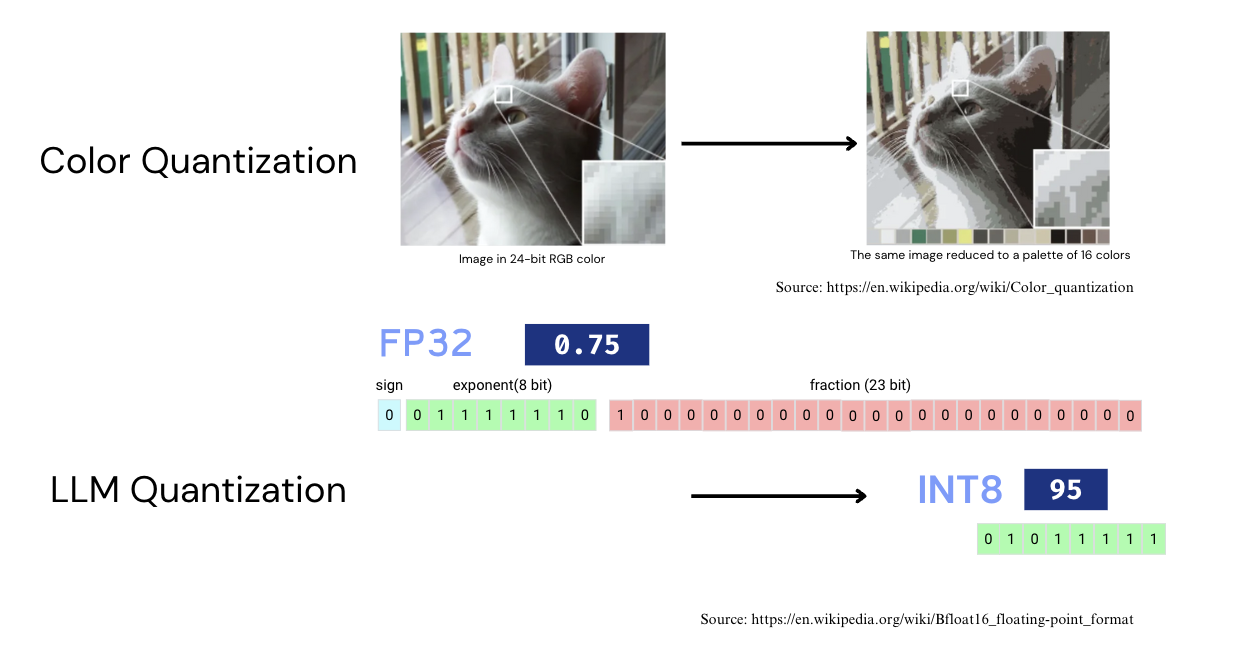
\includegraphics[width=\columnwidth]{img}
    \caption{Analogy between color quantization and LLM quantization}
    \label{fig:quantvisual}
\end{figure}

Quantization can be applied 1) during the training phase (\textit{QAT}) which is observed to be highly efficient; however, due to significant resource demands, oftentimes appears impractical \cite{chen2024EfficientQAT}, and 2) post-training (\textit{PTQ}), which is more resource efficient, but can lead to certain levels of performance degradation \cite{shen2024exploring}. An important quantitative marker of precision loss, quantization error, is often used to assess the degree of approximation loss \cite{lin2024AWQ}.

Having established the theoretical foundation of quantization, we now provide an overview of key methods. \textit{GPTQ} (Generative Pre-trained Transformers Quantization) focuses solely on weights and aims to minimize quantization error through optimal weight rounding. It is almost twice as effective as its one-shot predecessors and is capable of quantizing a 175 billion parameter model in a few hours with minimal accuracy loss\cite{frantar2023GPTQ}. \textit{AWQ} (Activation-aware Weight Quantization) assumes that weights carry varying levels of importance, therefore skipping crucial activation outliers while aggressively quantizing the rest helps mitigate accuracy loss. It also shows approximately 3x faster inference speed on a desktop, even allowing deployment and execution of a 13-billion model on a laptop with 8GB of RAM, which is of high interest for our study \cite{lin2024AWQ}. \textit{AQLM} (Additive Quantization of Language Models) is notable for achieving state-of-the-art optimization with extremely low-bit compression settings (as low as 2 bits per parameter), while still preserving high accuracy \cite{egiazarian2024AQLM}. The technique builds on the AQ (Additive Quantization) algorithm \cite{babenko2014additive}, but in contrast to the traditional approach, AQLM enables joint optimization of codebook assignment across layer blocks, referred to as \textit{additive quantization} in the paper. Although it is more computationally expensive, the authors provide efficient CPU and GPU implementations specifically designed for token generation tasks. Using these implementations, AQLM surpasses the study's baseline floating-point solution in inference speed, simultaneously reducing the memory usage by up to 8 times. \textit{SmoothQuant} \cite{xiao2023SmoothQuant} enables quantization for both activations and weights by managing outlier values and \textit{QLoRA} (4-bit quantized version of LoRA fine-tuning technique) \cite{dettmers2023qlora} reduces GPU requirements while still preserving performance.

The described approaches demonstrate not only superior advancements and efficiency, but are also feasible for us to experiment with. Therefore, in this study, we plan to access models from HuggingFace that have been quantized using the following techniques: GPTQ, AWQ, and AQLM. These approaches reduce model size\footnote{By ``size'' we refer to \textit{bit width} which in turn affects the memory needed for execution} to mitigate hardware requirements. Later we employ them to generate REST trace links, analyze their performance, and answer our RQs. 

\subsection{Cosine Similarity}
Cosine Similarity is an approach to determine how similar two text documents are based on the amount of shared words \cite{lahitani2016cosine}. By definition, it is computed as the cosine of the angle between two non-zero vectors, each of which corresponds to one of the two documents\cite{desku2021cosine}. Unlike LLMs, cosine similarity is a basic mathematical function that compares the content with no attention to semantic meaning. It relies on identifying the exact matching words, so even if two words are synonymous, they will be perceived as different and lower the similarity score. However, there are numerous preprocessing techniques that help normalize the data to achieve better performance. For example, using TF-IDF (Term Frequency–Inverse Document Frequency) \textit{smoothing}\footnote{TF-IDF is a technique used to identify the importance of a word within a document. Its value increases in proportion to the word’s frequency within the document (see: \href{https://tinyurl.com/mrfebkkt}{Scikit-learn documentation}. In this context, \textit{smoothing} refers to improvements made to the traditional approach, such as applying logarithmic scaling and adding constants making the technique more stable.} to better identify the importance of a particular word, as well as lowercasing and removing stopwords from text data.


\section{Research Methodology}\label{sec:method}

This section outlines the research type and its design (cf. Figure \ref{fig:method-overview}), and defines the scope pertaining to identified RQs. We structure our methodology section following the experimental process recommended by Wohlin et al. \cite{wohlin2012experimentation}. Furthermore, we explain and motivate the choice of methods and statistical tests for data analysis. 

We perform an \textit{experiment}, a research method commonly used to explore empirical correlations between several factors. Given the nature of  experiments, we gain control over subjects, objects, and instrumentation in order to operate on experimental units and draw conclusions on dependent variable output. Experiments are conducted to test the hypotheses and comparatively assess the impact of specific variables in a controlled setting, which is the most suitable setup for answering our RQs.

\begin{figure}[h]
    \centering
    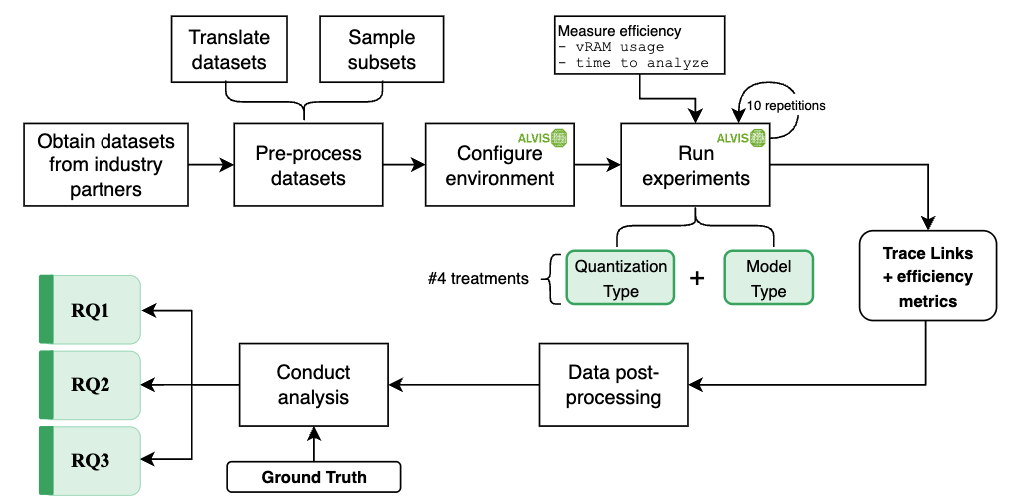
\includegraphics[width=\columnwidth]{images/method-overview-feedback}
    \caption{Overview of the research methodology process}
    \label{fig:method-overview}
\end{figure}

\subsection{Scope and Planning}
We define the scope of our experiment using the said framework of Wohlin et al. \cite{wohlin2012experimentation}. That is, we analyze quantized LLMs for the purpose of evaluation with respect to their efficacy, efficiency, and practicality from the point of view of practitioners in the context of industry REST alignment initiatives.

We conduct a controlled experiment to evaluate the effects of different quantization techniques. We select Mistral as a fixed model variable, with quantization techniques as a factor with four levels: \textit{None}, AQW, GPTQ and AQLM.

Our model selection is motivated by prior adoption in existing research as well as in industry. Moreover, the models (Mistral versions) are open-weight, which makes them accessible and transparent in contrast to proprietary alternatives (e.g., ChatGPT). Providers of proprietary LLMs generally do not disclose the internal structure of their models and usage of such models is accompanied by high execution costs. It is also worth noting that the study by Quinstedt and Lindgren \cite{quinstedt2024Optimizing} forms the foundation of our research and their discussion opened up the questions which we explore in our study. Aligning our model selection with theirs allows for a more nuanced and detailed analysis of the trade-offs associated with quantized model versions.

The dependent variables reflect the definition of performance in this study; they are: balanced accuracy, precision, recall, and F1-score (RQ1, efficacy), as well as time-to-analyze and GPU memory-usage (RQ2, efficiency).

Our control variables include a prompt template which yielded the the highest accuracy for our model selection in the previous study \cite{quinstedt2024Optimizing}, requirements specification and test case files, as well as mapping files---specifying the correct trace links between tests and requirements. 

\begin{figure}
    \centering
    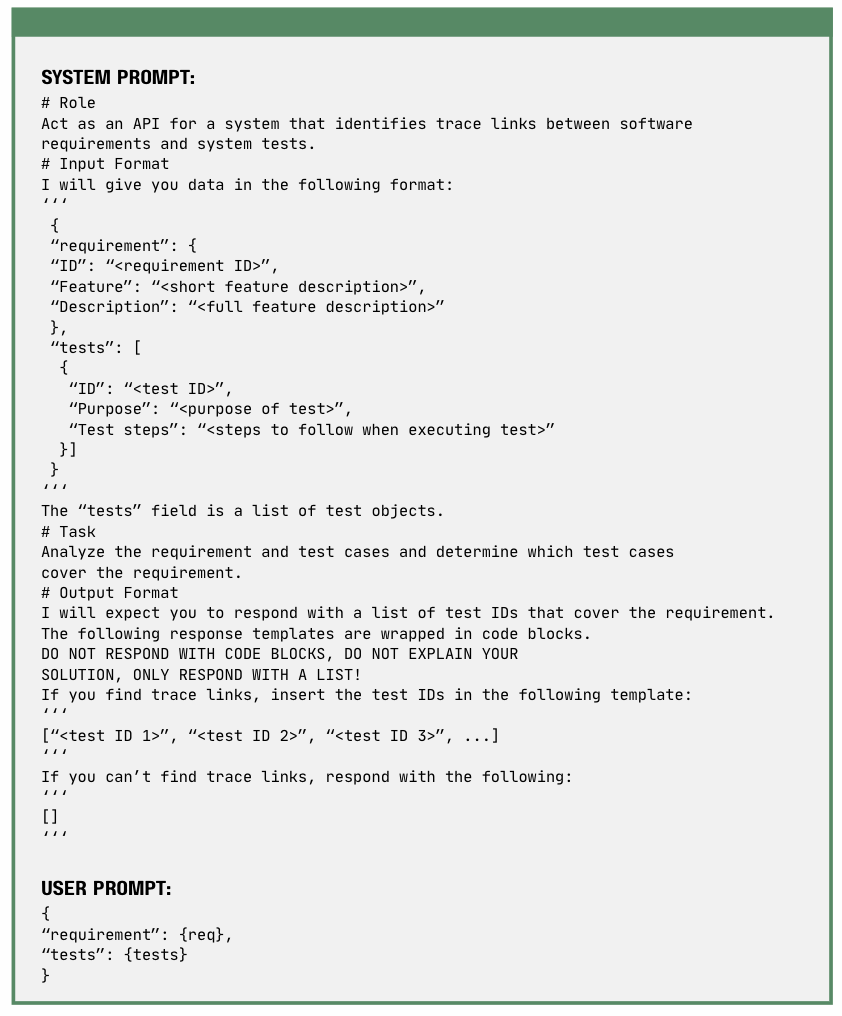
\includegraphics[width=\linewidth]{images/system_prompt}
    \caption{System Prompt Example}
    \label{fig:system_prompt}
\end{figure}

The datasets are as follows: \textbf{AMINA} has been provided to us by our industry partner and originates from G\"oteborg Energi, \textbf{BTHS} was sourced from Bluetooth Headset Profile 1.2\footnote{\url{https://www.bluetooth.com/specifications/specs/headset-profile-1-2/}}. In addition, we have web-scraped a public \textbf{Mozilla} test case repository\footnote{\url{https://www-archive.mozilla.org/quality/browser/front-end/testcases/}} and sourced the \textbf{Health Watcher} (HW) requirements document, containing the specification for a public health system, produced through a collaboration between academic and industrial practitioners\footnote{\url{https://zenodo.org/records/8081523}}

Tables \ref{tab:bths-hw}, \ref{tab:amina}, \ref{tab:mozilla} showcase the number of requirements (REs), software tests (STs) as of each dataset subset (sample), as well as the number of expected trace-links -- true-positives (derived from the respective ground truth file) and the maximal number of possible trace-links -- true-negatives\footnote{This is essentially $\text{REs} \times \text{STs}$ of that sample.}. We sample the datasets to reduce the overall computational costs in terms of time and to meet resource allocation constraints of the Alvis platform. Requirements are sampled from the full dataset and the connected tests are extracted to create subsets of 25 requirements with varying numbers of tests using Python's built-in PRNG function\footnote{Pseudo-random Number Generator, cf. \url{https://docs.python.org/3/library/random.html}}. However, since the sizes of BTHS and HW are smaller than the expected sample size of 25, we retain the original dataset without applying any sampling. Lastly, we also present the number of relationships between extracted REs and STs, specifying one-to-one ($1{:}1$), one-to-many ($1{:}M$), many-to-one ($M{:}1$), and many-to-many ($N{:}M$) trace-links, and the number of tests that no requirement is mapped to (labeled as ``unassigned'').

Furthermore, model hyper-parameters are kept constant and configured consistently across different models. For instance, we set \textit{temperature = 0.1} to control the randomness of the LLM output; a lower value makes the output more deterministic.

An overview of the experimental design can be found in Figure \ref{fig:exp-design}. See subsection \ref{sec:instrumentation} for further specification of the experiment objects.

%%%%%%%%%%%%%%%%%% HYPOTHESIS TABLE %%%%%%%%%%%%%%%%%%

\newcommand{\equalM}{$M_{1} = \dots = M_{4}$}
\newcommand{\notEqualM}{$M_{1} \neq \dots \neq M_{4}$}

\begin{table}[h]
    \centering
    \caption{Experiment Hypotheses}
    \renewcommand{\arraystretch}{1.65} % original value 1.5
    \begin{tabular}{@{} c p{3.5cm} p{3.5cm} @{}}
    \toprule
    &\multicolumn{1}{c}{\textbf{(i) Efficacy RQ1}}
    &\multicolumn{1}{c}{\textbf{(ii) Efficiency RQ2}} \\
    \midrule
    $H_{0}$ % <-- NULL HYPOTHESIS %
    & There is no difference in \textbf{efficacy} between the treatments
    under test; \equalM.
    & There is no difference in \textbf{efficiency} between the treatments
    under test; \equalM.\\
    $H_{a}$ % <-- ALT HYPOTHESIS %
    & There is a difference in \textbf{efficacy} between the treatments
    under test; \notEqualM.
    & There is a difference in \textbf{efficiency} between the treatments
    under test; \notEqualM.\\
    \bottomrule
    &\multicolumn{2}{c}{Note: the individual treatments are labeled as $M_{1\dots4}$.} \\
    \end{tabular}
    \label{tab:hypothesis}
\end{table}

\subsubsection{Baseline Solution---Cosine Similarity Algorithm}

Previous research on the use of LLMs for REST alignment did not compare their performance against a baseline solution. Therefore, we choose the \textbf{cosine similarity algorithm} for this purpose. We apply the following optimization techniques: text pre-processing, stop word removal, and TF-IDF vectorization. We use the balanced accuracy metric to accurately assess and compare the performance of this technique with the LLMs results.

\subsection{Data Collection}\label{sec:data-collection}

First, we collect data and derive metrics from repeated test iterations. The process is repeated with 10 repetitions per treatment per dataset (or one repetition per each dataset subset---if they exist, in which case there are ten). We altogether obtain $4 \times 4 \times 10 = 160$ output artifacts, which are result files containing generated trace links and benchmark data in a \verb|JSON| format. When analyzing the data, we initially examine the treatments from two perspectives: (i) efficacy, and (ii) efficiency---evaluating the null hypotheses for these groups of metrics separately (cf. Table \ref{tab:hypothesis}).

Note that, given the stochastic nature of LLMs, it is important that we perform repeated tests on each of the treatments in order to include standard deviation measurements across the different metrics. This also allows us to reason about the consistency of each treatment as well as increase the validity of our measurements and subsequently the results of our analysis.

On the other hand, given to the deterministic nature of the baseline algorithm, we execute it once on each complete dataset to retrieve the corresponding similarity scores. We calculate the balanced accuracy values using the same formula applied in a confusion matrix.


%%%%%%%%%%%%%%%%%% EXPERIMENTAL DESIGN FIGURE %%%%%%%%%%%%%%%%%%

\begin{figure}[h]
\begin{center}
    \begin{tcbraster}[raster columns=2, raster column skip=5pt, raster equal height=rows, raster row skip=5pt]
        \begin{roundedBox}
            \centering
            \textbf{Independent Variables \& Levels}
            \begin{itemize}
                \item Quantization technique:
                \begin{itemize}
                    \item None
                    \item GPTQ Quantization
                    \item AWQ Quantization
                    \item AQLM Quantization
                \end{itemize}
            \end{itemize}
        \end{roundedBox}
        \begin{roundedBox}
            \centering
            \textbf{Objects}
            \begin{itemize}
                \item Hardware (Alvis)
                \item Alvis job-scripts
                \item REST-at tool
                % \item Hardware: local
            \end{itemize}
        \end{roundedBox}
        \begin{roundedBox}
            \centering
            \textbf{Dependent Variables}
            \begin{itemize}
                \item Balanced Accuracy
                \item Precision
                \item Recall
                \item $F1$-score
                \item Time-to-analyze
                \item GPU memory-usage (VRAM)
            \end{itemize}
        \end{roundedBox}
        \begin{roundedBox}
            \centering 
            \textbf{Control Variables}
            \begin{itemize}
                \item Model (Mistral)
                \item Requirements file
                \item Test case file
                \item Ground truth file
                \item Prompt template
                \item Model hyper-parameters
                \item Python environment (version)
            \end{itemize}
        \end{roundedBox}
        \begin{roundedBox}
            \centering
            \textbf{Blocked Variables}
            \begin{itemize}
                \item Dataset:
                \begin{itemize}
                    \item AMINA
                    \item BTHS
                    \item Mozilla
                    \item HW
                \end{itemize}
            \end{itemize}
        \end{roundedBox}
        \begin{roundedBox}
            \centering
            \textbf{Output (artifacts)}
            \begin{itemize}
                \item Result file, containing:
                \begin{itemize}
                    \item Structured trace links
                    \item Benchmark data
                \end{itemize}
            \end{itemize}
        \end{roundedBox}       
        \end{tcbraster}
    \caption{Overview of the experimental design}
    \label{fig:exp-design}
\end{center}
\end{figure}

\subsection{Instrumentation}\label{sec:instrumentation}
For our instrumentation, we extend \verb|REST-at| by adding support for (i) quantized models, and (ii) logging efficiency benchmark data from the models' execution. We run our experiment on Alvis, a cloud platform for scientific computing. The system is built around NVIDIA GPUs, and allows executing jobs on demand. Therefore, we execute the experiment on a dedicated NVIDIA A100 Tensor Core GPUs\footnote{\url{https://www.nvidia.com/en-us/data-center/a100/}}, hence are all gathered performance and efficiency metrics based on this hardware configuration.

For our experiment, we require a set of requirements linked with a corresponding set of tests. The datasets with trace links serve as \textit{ground truth} since these are established by the authors from the companies.

\subsection{Analysis and Interpretation}\label{sec:analysis}

% FROM METHOD SCOPE - REMOVED
% After testing for our null and alternative hypotheses, we apply a post-hoc pairwise comparative analysis of the treatment pairs. Finally, a descriptive analysis investigates trade-offs of using quantized LLMs for REST alignment; we combine the results from both efficacy and efficiency metrics, as well as some additional factors (e.g., implementation challenges, learning curve) that are described in detail in subsection \ref{sec:analysis}.

The data analysis includes performance indicators from a confusion matrix, namely in terms of balanced accuracy, precision, recall, $F_1$-score (see below). Those measures convey the efficacy of the treatment under test. We use descriptive statistics and data visualization to identify differences between the treatments. 

\begin{table}[h]
    \centering
    \caption{Evaluation Metrics in the context of REST}
    \begin{tabular}{@{}ll@{}}
    \renewcommand{\arraystretch}{1.5}
    \toprule
    \textbf{Metric} & \textbf{Definition} \\
    \midrule
    Positive (P) & A trace-link between a requirement and a test.\\
    Negative (N) & Absence of a trace-link between a requirement and a test.\\
    True positive (TP) & A correctly detected existing trace-link. \\
    True negative (TP) & Omission of an existing trace-link. \\
    False positive (TP) & A correct detection of an absence of a trace-link. \\
    False negative (TP) & Incorrect detection of a non-existent trace-link. \\
    \midrule
    Prevalence & $\frac{P}{P + N}$ \\
    Accuracy & $\frac{TP + TN}{P + N}$ \\
    Balanced accuracy & TODO \\
    Precision & $\frac{TP}{PP}$ \\
    Recall & $\frac{TP}{P}$
    $F_1$-score & The harmonic mean of the precision and recall. \\
    \bottomrule
    \end{tabular}
    \label{tab:eval-metrics-def}
\end{table}

\begin{table}[h]
    \centering
    \caption{Confusion Matrix}
    \begin{tabular}{|c|c|c|c|}
    \hline
    \multicolumn{2}{|c|}{} & \multicolumn{2}{c|}{Predicted condition} \\
    \cline{3-4}
    \multicolumn{2}{|c|}{Population} & Positive (PP) & Negative (PN) \\
    \multicolumn{2}{|c|}{= P + N} & & \\
    \hline
    \multirow{2}{*}{\begin{tabular}{c}Actual\\condition\end{tabular}} & Positive (P)\vphantom{Ag} & True positive (TP) & False negative (FN) \\
    \cline{2-4}
    & Negative (N)\vphantom{Ag} & False positive (FP) & True negative (TN) \\
    \hline
    \end{tabular}
    \label{tab:confusion_matrix}
\end{table}

A tabular layout comparing actual class with instances of a predicted class 

Our full factorial design has two factors. The data is paired as we will be comparing the same data points (rows) between different treatments. First, we will analyze the distribution of the collected data. Specifically, we will use the Shapiro-Wilks test to check for distribution normality and Levene's test to check for homoscedasticity---equal or similar variance between groups. If these tests show that necessary assumptions are met, we will use a parametric two-way ANOVA statistical test. If the assumptions do not hold, we will instead use a non-parametric Friedman test which is an alternative to repeated ANOVA-measures \cite{mccrum2008statisticalTests}.

Should the null hypothesis be rejected, indicating that there is a significant difference between at least one of the treatment pairs, we conduct a pairwise post-hoc analysis to identify the differing pairs as well as in which direction they differ. By evaluating the treatment pairs, we can examine whether certain quantization techniques result in better model performance within the given context. 
%The z-score based Dunn's test will be used for the post-hoc analysis, as the sample size is $>$30 \cite{dunn1964dunnTest}. 
% Can also mention that it is a rank-based follow-up test to Kruskal-Wallis - if we can find a source ... -_-
% ...or the Conover-Iman test \cite{conover1979conoverImanTest} will be used depending on the sample size. 
% NOTE: keeping this here since we might use this test instead (it has better statistical power)? Also, is it okay that we cite the original sources here and not literature that recommends the test's usage?
We use the Holm–Bonferroni method to mitigate \textit{alpha inflation} which would otherwise increase the risk of type I errors---while also reducing the risk of type II errors compared to the regular Bonferroni method \cite{abdi2010HolmBonferroni}.
We will choose between t-test (parametric) or Mann-Whitney (non-parametric), depending on the distribution of the resulting data - BUT when the report is published we will have already made this decision, so this is probably unnecessary to state

% We conduct a descriptive statistical analysis of the results to analyze and discuss the trade-offs of applying quantization to LLMs within the given context.
Ultimately, we are interested in examining whether there exists any treatment(s) that retains acceptable / usable recall and F1-score results despite significantly reducing GPU memory-usage. Thus, we combine the efficacy and efficiency metrics alongside the following additional factors: implementation challenges, learning curve, model VRAM usage compared with commercial GPU alternatives, cost comparison of manual and automatic solutions. 

We choose to represent the data in tables comparing the results from the different treatments. For this purpose, \textit{mean $\pm$ standard deviation} is displayed for each of the relevant metrics. We also select box-plots in order to visualize the distribution as well as any outliers in each treatment's performance. Lastly, we use bar charts to give a clear comparison of the performance as a result of the different quantization techniques.

\section{Results}

This section presents our findings according to the research questions posed in this study.

\begin{figure}[H]
    \centering
    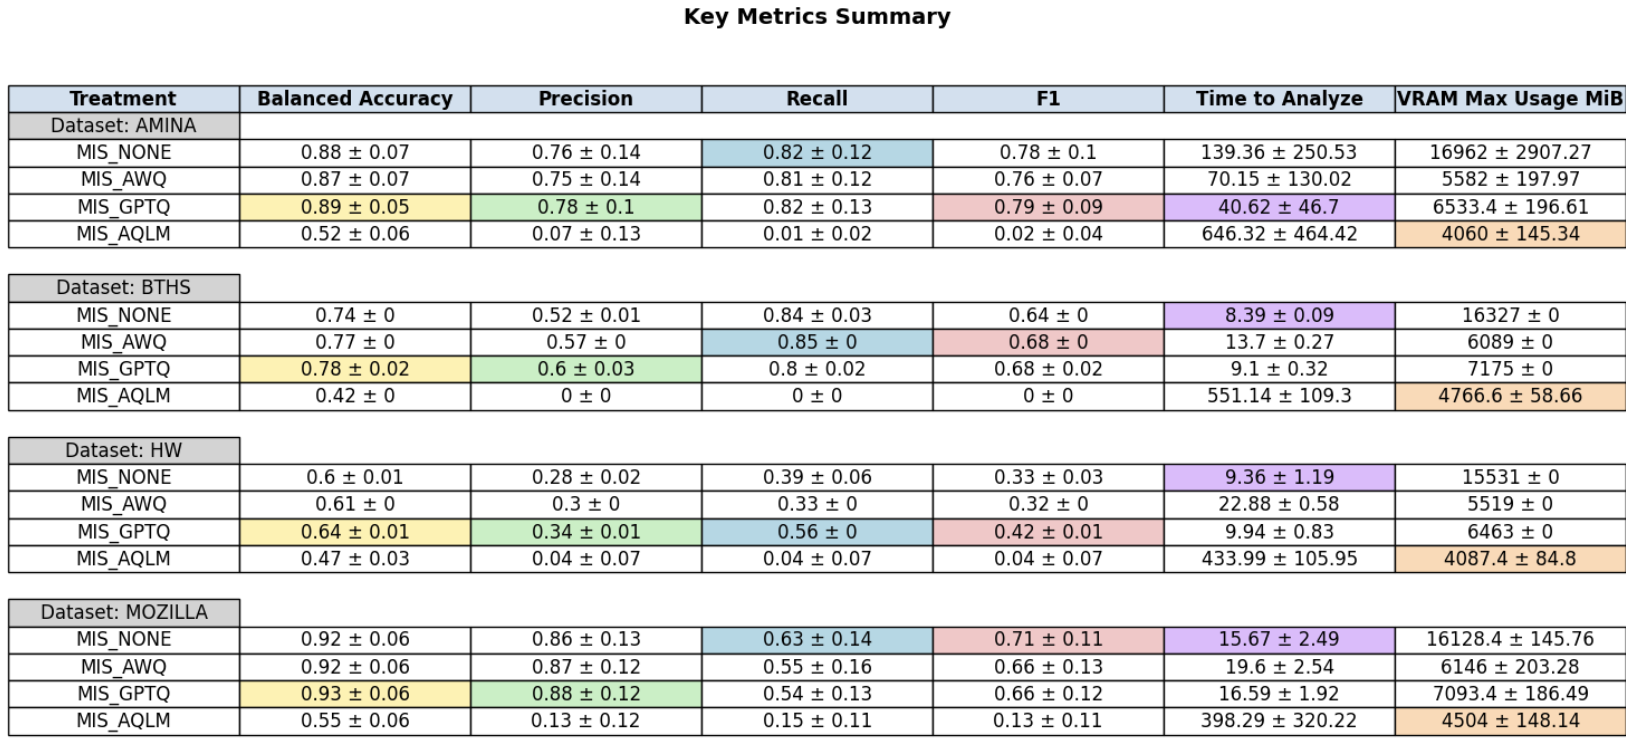
\includegraphics[width=0.95\columnwidth]{images/MVP_summary_table.png}
    \caption{MVP summary table}
    \label{fig:mvp-table}
\end{figure}

In this table we compare the effects of different quantization techniques across all datasets in terms of metrics for RQ1 (balanced accuracy, precision, recall, F1) and RQ2 (Time to Analyse and VRAM usage).
 
Quantization generally led to reductions in both VRAM usage and inference time, but the results reveal several significant observations in regards to the quality of the output.

Notably, GPTQ consistently offers the best trade-off between performance and accuracy among all datasets. It persistently matches or improves on the baseline F1 score (e.g., Amina: NONE: 0.78 ± 0.09, GPTQ: 0.79 ± 0.01.; BTHS: NONE: 0.64 ± 0, GPTQ: 0.68 ± 0.02). It reduces VRAM on average by \>40\% compared to baseline NONE treatment. Moreover, no dataset shows severe degradations, supporting its reliability.

In contrast, AQLM significantly reduced memory consumption (on average, 3,5 times), however it often falls short in recall and F1 score(e.g. 0 on BTHS, and not higher than 0,11 on the other data). The result is probably a consequence of AQLM's aggressive 2-bit quantization, which led to significant information loss and decreased the usability of the model for this use case.

AWQ results appear to be neutral, its gains in optimized resourced do not correlate to high accuracy. AWQ results occasionally outperform the base NONE model (e.g. BTHS )and performance is slightly lower than GPTQ in most cases.


Naturally, NONE model has the highest memory and resources demands, but

 In addition, there is a correlation between the dataset size, complexity and results ...
talk about mozilla 


 

\subsection{\textbf{RQ1:} efficacy of quantized LLMs for creating REST links}

\begin{figure}[H]
    \centering
    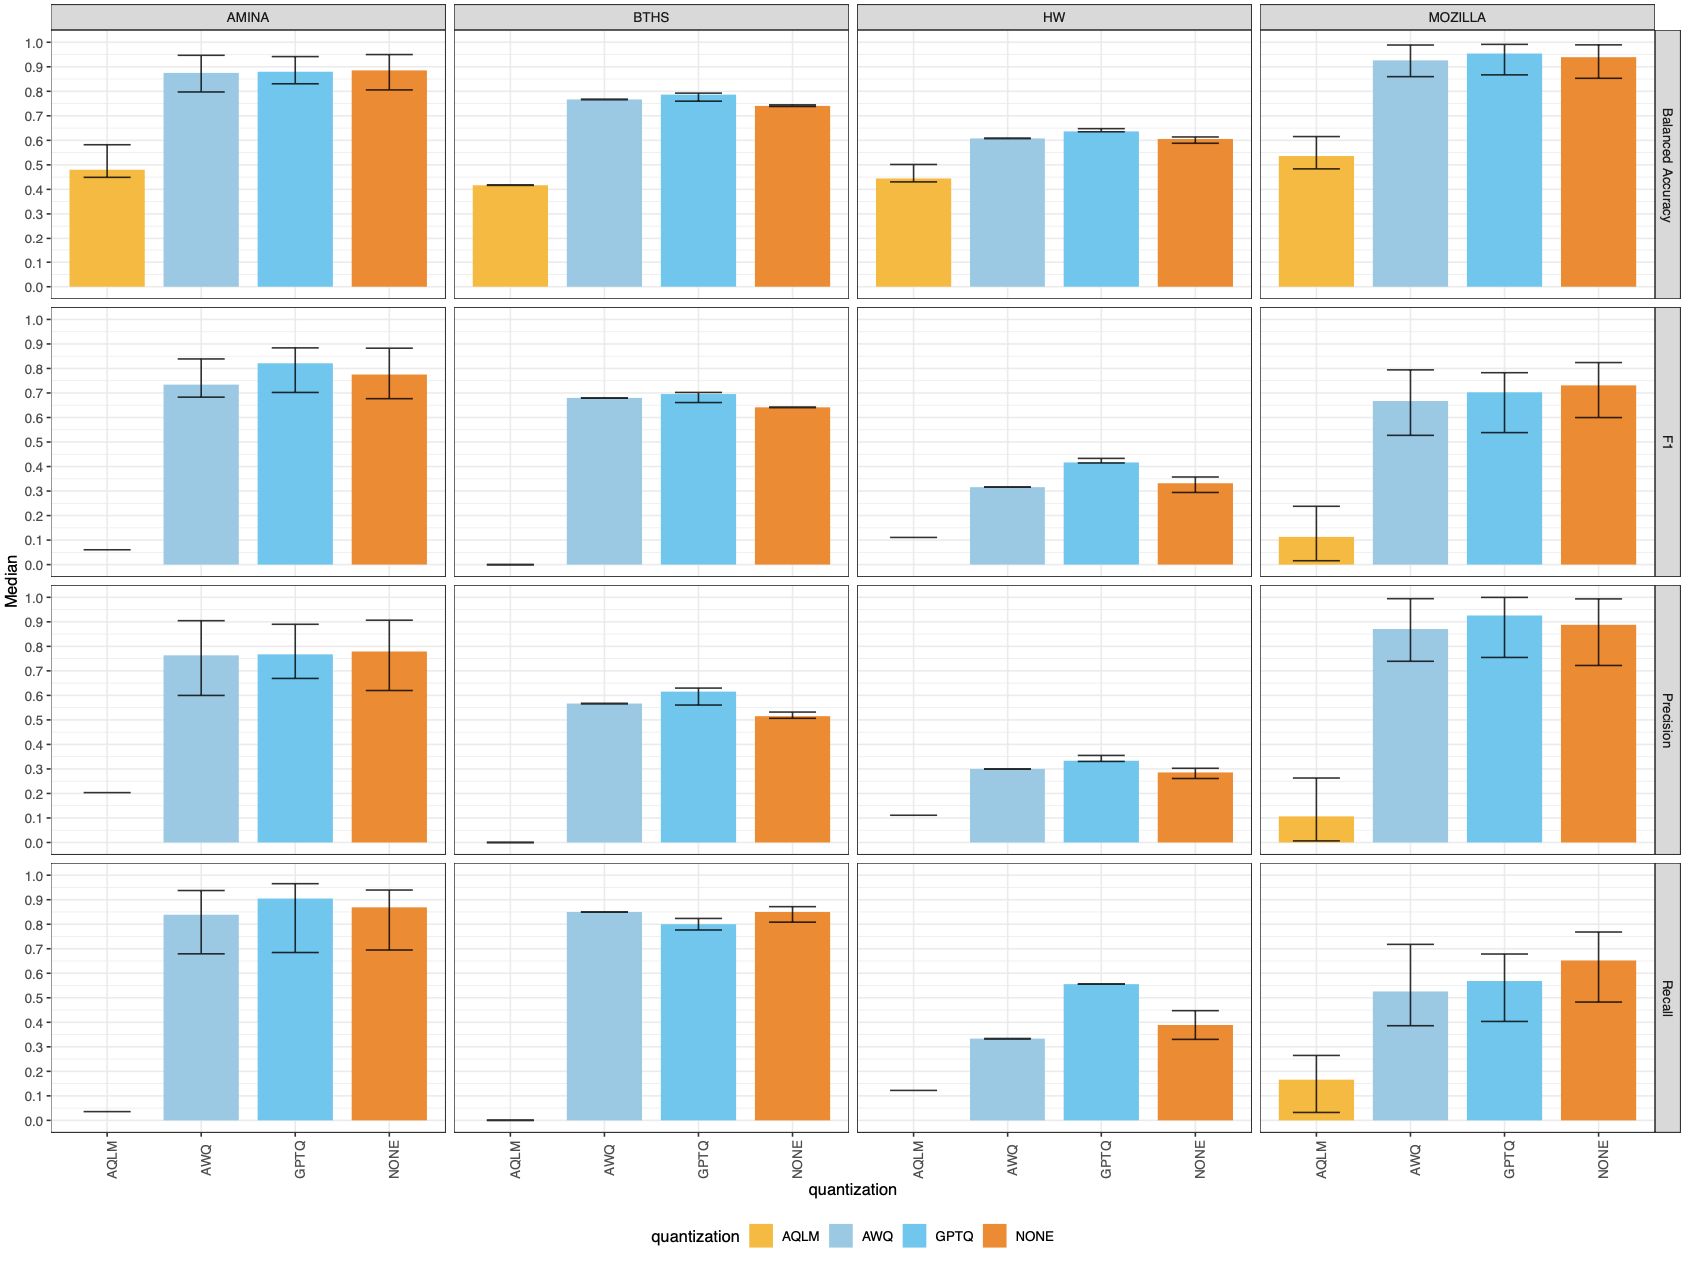
\includegraphics[width=0.99\columnwidth]{images/RQ1_quant_comparison.png}
    \caption{RQ1}
    \label{fig:rq1}
\end{figure}

\subsection{\textbf{RQ2:} efficiency of quantized LLMs for creating REST links}

\subsection{\textbf{RQ3:} trade-offs of using quantized LLMs with respect to efficacy versus efficiency}

\subsection{Baseline solution --- Cosine Similarity}

The results achieved on the tested datasets using cosine similarity algorithm are presented in the Table X. There is a correlation between the datasets that containing a consistent set of keywords and obtaining high results, in contrast datasets with more complex and varied language, scored significantly lower. In particular, BTHS, has entries in the dataset with a lot of overlapping text (that is, RE contains many keyowrds also found in the test cases) hence obtaining the highest accuracy (87.50\%). 

The language for the other datasets is more varied and manytimes synonym are used to describe a certain phenomenon (maybe take example from Mozilla) which the algorithm will struggle with.

\begin{table}[h]
    \centering
    \caption{Cosine Similarity Score Baseline Accuracy\label{tab:cosine_baseline_accuracy}}
    \renewcommand{\arraystretch}{1.2}
    \begin{tabular}{||l|c||}
    \hline
    \textbf{Dataset} & \textbf{Balanced Accuracy (\%)} \\
    \hline
    BTHS & 68,5\% \\
    AMINA & 97,34\% \\
    Mozilla & 93,91\% \\
    HealthWatcher & 86,8\% \\
    \hline
    \end{tabular}
\end{table}


\begin{figure}[H]
    \centering
    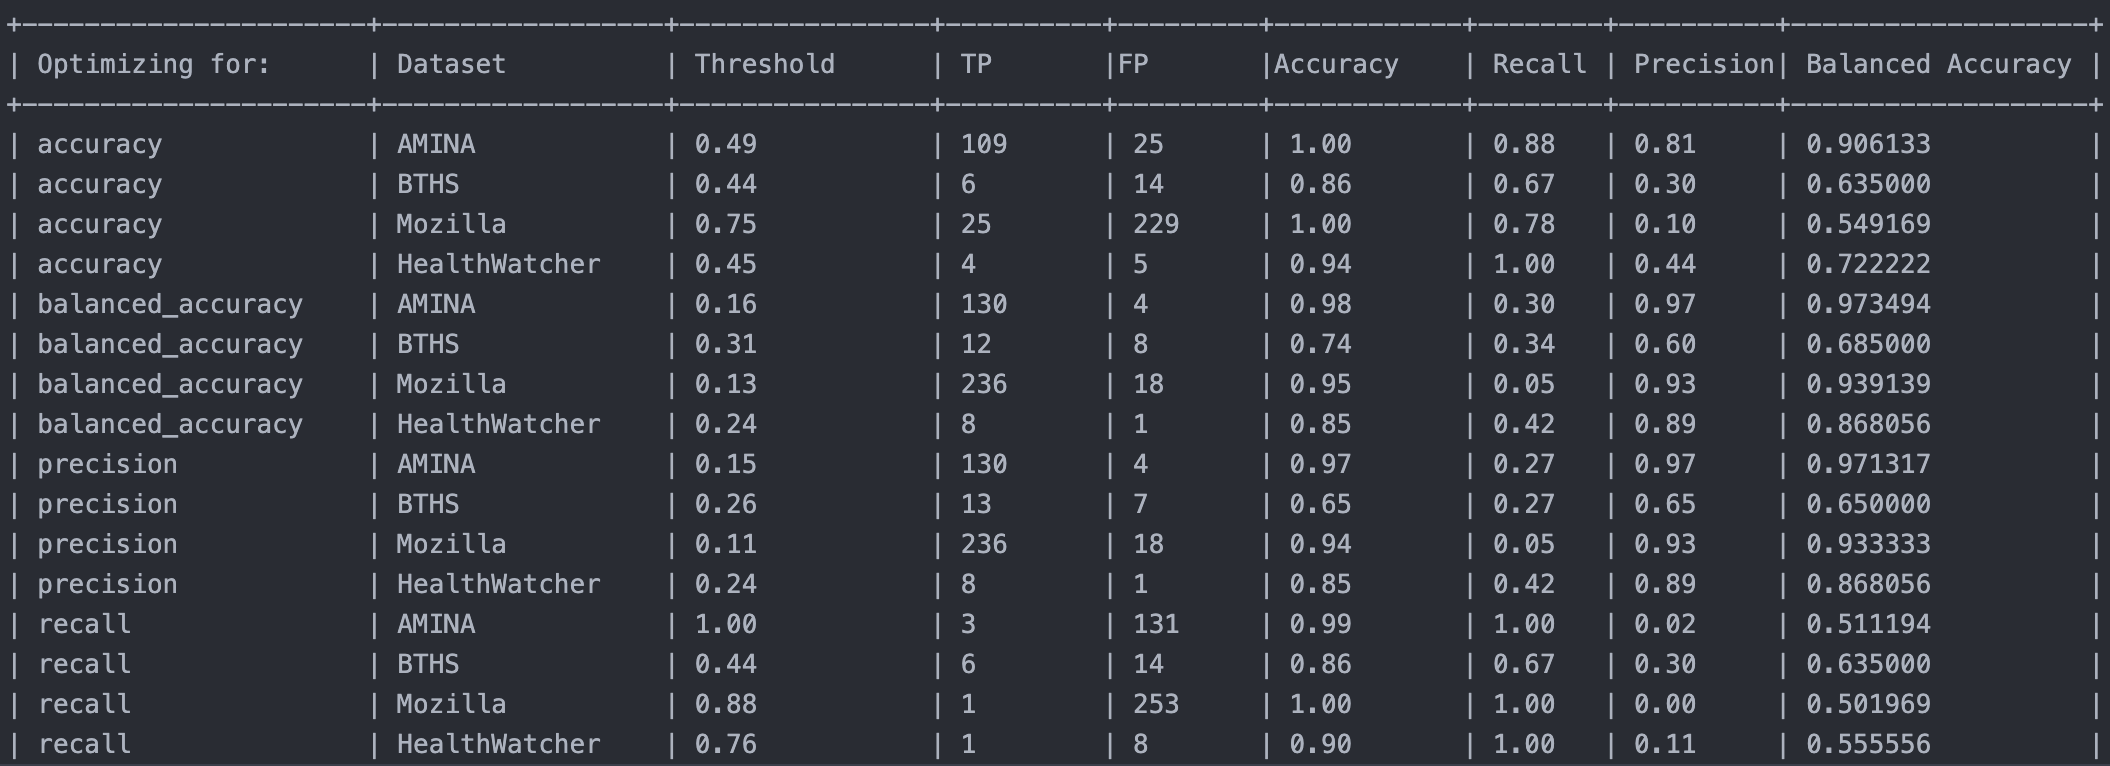
\includegraphics[width=0.99\columnwidth]{images/cosine_confusion_matrix.png}
    \caption{Confusion Matrix for Cosine Similarity algorithm}
    \label{fig:confution_cosine}
\end{figure}


\section{Discussion}

In this section, we delve into the implications of our findings and relate them to existing research. We aim to provide a comprehensive analysis of the contextual factors and challenges that influence and frame our findings. 

\subsection{Feasibility of using quantized LLMs for REST}

RQ3: implementation challenges, learning curve,
ALL OF THEM

GPU costs vs. model performance vs. developer salary if manual work vs. ...


\subsection{Challenges in adopting quantized LLMs for local use}

While it is fascinating to observe how rapidly technology develops nowadays, it also establishes the requirement to keep pace with rapid updates. Sometimes, frequently introduced updates to the libraries disrupt previously functioning code resulting in additional debugging effort.

Moreover, we have also observed that even despite having a well-defined prompt structure, not all quantized models adhere to these standards when providing response. For instance, AQLM repeatedly produced results in such format (Example). This discrepancy leads to additional parsing, increasing complexity and reducing the overall usability of such models.

For heavier models (Llama, Mixtral), quantization still may not reduce it to a fully usable level unless you don't have a beefy GPU. Mention how we were struggling with this even on Alvis.

Similarly as for non-local use, the ever-changing dependencies that may cause conflicts could be pairsed with system-specific issue (e.g., Cuda kernel configs) that could greatly diminish the development perspective and, above all, the usability.

Each model required a separate environment setup and extensive configuration. For instance, we provisioned an entirely new Ubuntu machine for AQLM setup and faced many issues along the way. However, it ultimately led to a situation where the time and effort invested in configuration were not justified by the obtained results.

We still need to wait more for models to be run seamlessly on a regular dev computer. Also many users have non-INTEL-based GPUs, particularly the M mac series have become increasingly popular, and, then, the native support for Nvidia tools is impossible, and alternative solution would need to be employed. Despite the newly introduced Apple's Metal API (https://developer.apple.com/metal/), the technology is rather new and is being still worked on and implemented, and users continue to report integration issues to this day.

% I want to say that even though there's more stuff becoming available, it's still quite unstable, and things break all the time, especially on mac, windows, intel/metal, etc.

Moreover, we have observed that the size of the data set significantly influences the performance of models. In particular, we have initially set up the experiment with the sample size of 100 entities. However, it was not feasible to run the entire experiment using the full data sets. From the practical point of view, it appeared more realistic to proceed with data samples of 25 rows per document, which led to significantly better results.


The VRAM consumption is affected by the size of the text that the model receives. That is, each input sequence is turned into tokens, and the tokens in turn get translated to activation tensors and possible caches. More text, more to process, more resources needed. This is during inference, i.e. after the model is loaded and the user provides a text input sequence. This can be seen in the avg. VRAM usage of the experiment.

Notice that Mozilla has the higest average VRAM consumption. That is, because the prompt (text) received on the dataset is the longest. Note that 1 token is typically ca. 4 chars in English.

PT6 consists of (i) system prompt: 992chars, (ii) user prompt: 27 chars. Maybe update this?
Calculation: the prompt template has a fixed size of ~500 characters. Based on the template provided above, each prompt consists of:

\verb"<PROMPT>REQ: {ALL_TESTS}<PROMPT>"

A requirement consists of the feature and description and a test consists of a purpose and test steps. Each prompt shows one requirement and all possible test cases it can map to.

We've determined the average string lengths of these columns of each dataset

\begin{table}[h]
    \centering
    \caption{Dataset string sizes distribution (char)}
    \begin{tabular}{||p{1.65cm}|p{1.1cm}|c|p{1.1cm}|c|p{0.75cm}||}
    \hline
    Dataset & \# of REs, STs & Feature & Description & Purpose & Test steps \\
    \hline
    AMINA         & 100, 130 & 27.54 & 153.32 & 32.59  & 172.12 \\
    BTHS          & 8, 15    & 33.75 & 487.50 & 103.67 & 677.80 \\
    Mozilla       & 316, 254 & 18.92 & 81.41  & 103.34 & 663.65 \\
    HealthWatcher & 9, 9     & 16.89 & 177.44 & 0      & 996.78 \\
    \hline
    \end{tabular}
\end{table}

Then for each dataset, an average prompt string size is determined by fixed template size + average requirement string size + (sample size * average test string size). We set sample size to 25, but on datasets with less entries (BTHS, HealthWatcher), we consider the whole datasets (guaranteed to be $\leq 25$).

Putting this altogether, we get that the average prompt string sizes are:

\begin{table}[h]
    \centering
    \caption{Average prompt string size}
    \begin{tabular}{||c|c|c|c|c|c||}
    \hline
    Dataset & $\approx$ \# of chars \\
    \hline
    AMINA         & 5,817 \\
    BTHS          & 12,761 \\
    Mozilla       & 19,794 \\
    HealthWatcher & 9,683 \\
    \hline
    \end{tabular}
\end{table}


\subsection{Challenges in Designing the Experiment}
	% - Watchdog complains and quits the job if the usage of GPU is too low
 %    - Setting up GPU-Profiling was difficult, started with scalene, but then went for nvidia-smi as it is natively supported by alvis
	% - We were scheduling jobs on Alvis and they have a queue-based system. When the platform is busy, it’s very hard to get the time to run. However, it’s generally easier to get A100 than A100fat GPU

% * Discuss some (technical) "failures"/ decisions. E.g. why we omitted GGUF? Why we didn't use scalene?
% * Relation to baseline? Flow-chart diagram. Which is better under what conditions?


\subsection{Choosing Between Cosine Similarity and LLMs}

As we have discussed, the cosine similarity algorithm is a lightweight yet powerful solution in the case of a substantial overlap in text among the files. However, it faces significant limitations with respect to semantic understanding. Based on our findings, we provide guidance on the scenarios in which this technique may be applicable.

\textbf{General recommendation:} Carefully review your data to identify if the requirement and test specification consistently uses a set of keywords with little to no variations in phrasing. If so, Cosine Similarity can serve as a light-weight solution to experiment with. Otherwise, consider testing LLMs.

Please consider the following steps or conditions to navigate your choice:

\begin{figure}[H]
    \centering
    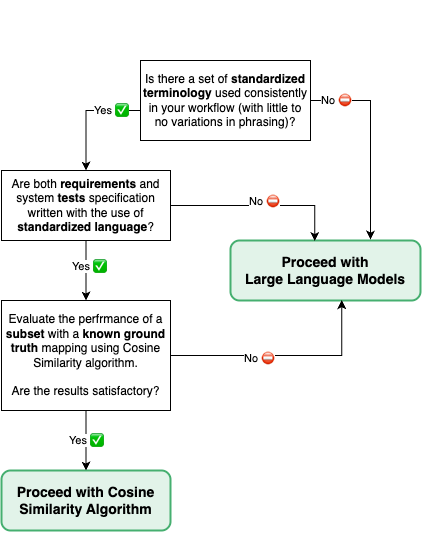
\includegraphics[width=0.75\columnwidth]{images/flowchart.png}
    \caption{Flowchart Illustrating Method Selection Guidelines}
    \label{fig:flowchart}
\end{figure}

%===== DATA SAMPLES ======


Here is the example of RE(requirement)-ST(test) pairs from the AMINA dataset that scored 86\% mapping correctness in our experiment: 

\textbf{AMINA}
  \begin{databox}
    RE: B102,Retrieve meter reading data for 24h for 95\% of meters within 60 min,The communication solution should be able to collect 95\% of all measurement data from 400 000 meters and for the latest 24 hours within 60 minutes.
    ST: 378,Retrieve meter data for 24 hours for 95\% of meters within 60 minutes,"Verify that the communication solution can retrieve 95\% of all measurement data from 400,000 meters and for the past 24 hours within 60 minutes."
    Mapping: B102,378
\end{databox}


 \begin{roundedBox-sm}
    \textbf{RE:} B107,Version control of web service interfaces,Web service interfaces should (B107) be version controlled so that old versions can be used if necessary.
    
    \textbf{ST:} 25,Version control of web service interfaces,Verify that the previous version of the web service interface can be read back and is compatible with the new version or previous version of ACM.
    
    \textbf{Mapping:} B107,25
\end{roundedBox-sm}

Here are some examples of other datasets that have been utilized.

\textbf{BTHS}
 \begin{roundedBox-sm}
    \textbf{RE:} 4.6.1,Audio Connection Transfer from AG to HS,"The audio connection transfer from AG to HS is initiated by a user action on the HS side. To effect this transfer, the HS shall send the AT+CKPD=200 command to the AG."
    
    \textbf{Tests:} HSP/AG/ACT/BV-01-I,"To verify that the AG can perform an audio connection transfer from AG to HS initiated by a user
action on the headset.","Initial condition: 
- Both devices are initilized. Ensure HS and AG are initially paired, confirming interoperability for the headset profile. 
- HS is in Standby mode, no connection to AG
- For AG a call/audio connection is active at the AG.

Procedure: 
HS: Initiate the user action (e.g. press button) on the HS to transfer the audio connection from AG to HS
AG:No user action is required
  
Expected Outcome AG:The user action on the HS transfers the audio connection from AG to HS"
    
    \textbf{Mapping:} 4.6.1,HSP/AG/ACT/BV-01-I
\end{roundedBox-sm}

\textbf{Health Watcher}
 \begin{roundedBox-sm}
    \textbf{RE:} FR15,Update health unit,This use case allows the health unit's data to be updated.
    
    \textbf{ST:}T-8,,"1. The employee chooses the update health unit option.
2. The system retrieves the list of all health units.
3. The list of health units is returned to the employee.
4. The list of health units is formatted and displayed on the employee’s local display.
5. The employee selects the health unit to be updated.
6. The unique identifier for the selected health unit is sent to the server.
7. The system ensures the health unit data is consistent.
8. The system retrieves the data for the selected health unit.
9. The data retrieved is returned to the employee.
10.The health unit data is formatted and presented on the employee’s local display.
11.The employee alters the necessary data.
12.The updated information is sent to the server.
13.The system ensures the health unit data is left in a consistent state. 
14.The system stores the updated health unit information."
    
    \textbf{Mapping:} FR15,T-8
\end{roundedBox-sm}

\textbf{Mozilla}

\begin{roundedBox-sm}
    \textbf{RE:} R-005,Double-clicking on a bookmark shall cause it to be launched in a browser window.,Double-clicking on a bookmark shall cause it to be launched in a browser window.

    
    \textbf{ST:} TC-005,,"INITIAL CONDITIONS
1. You must have a bookmarks file.
2. To promote consistency, you may choose to use the default set of Netscape Seamonkey Bookmarks.
3. You also have the option to use this very large bookmarks file.
4. You must also customize your sidebar to include a bookmarks panel.

STEPS/DESCRIPTION
1. Select the toplevel ""Bookmarks"" menu. Select any bookmark on the list.
2. Click ""Bookmarks"" on the Bookmarks/personal toolbar. Select any bookmark on the list.
3. Open the sidebar; click on the ""Bookmarks"" panel. Double-click any bookmark on the list.
4. From the toplevel ""Bookmarks"" menu select ""Manage Bookmarks"". Double-click any bookmark in the window.

EXPECTED RESULTS
In all cases, the url corresponding to the bookmark you selected should be loaded in the browser window.

LINKS
1. default-bookmarks.html
2. large-bookmarks.html"

    \textbf{Mapping:} R-005,TC-005

\end{roundedBox-sm}

\subsection{Threats to Validity}
% - Describe internal validity threats and mitigations.
% - Describe construct validity threats and mitigations.
% - Describe external validity threats and mitigations.
% - If applicable for your research method, describe further validity threats and mitigations under further categories.

Based on the guidelines proposed by Wohlin et al. \cite{wohlin2012experimentation} we identify the following threats to validity that might have influenced our research findings: 

\subsection*{\textbf{1) Internal Validity}}

\textit{Response variability}: due to stochastic behavior of LLMs, the same prompt can result in different outputs when executed several times; we mitigate this risk by invoking prompts multiple times and defining consistent hyperparameters.

\textit{Selection of Models}: in this study, we select open-weight, state-of-the-art LLMs representative of a common choice among practitioners. This selection also leverages on the previous research by Quinstedt and Lindgren \cite{quinstedt2024Optimizing}, which we are building on. Aligning the selection of LLMs with their results allows for a more extensive and direct trade-off comparison. More models can be explored in future work, and we provide instrumentation in the Methodology section to facilitate the smooth integration.

\textit{Quantized LLM Quality}: we have utilized quantized models distributed via the \textit{HuggingFace} platform. While there is a risk in depending on quantized models from a third-party service, HuggingFace is one of the main sources for developers or organizations to download and/or deploy open weight models. As such, these models are likely to be used by practitioners, meaning that the results of our study are representative of the real-world use of quantized LLMs, given that this assumption holds.

\textit{Target Bit-widths}: Quantization techniques typically offer configurable target bit-widths to adjust the aggressiveness of the algorithm, influencing the amount of information lost from the original model. To comprehensively assess the impact of the selected quantization techniques it is necessary to explore several target bit-width levels for the models under test. However, due to scope limitations, this study focuses on a higher-level comparison of quantization techniques and does not encompass a broader range of target bit-widths. 

\subsection*{\textbf{2) External validity}}
    
\textit{Domain-Specific Applicability}: our study evaluates quantized LLMs within the specific use case of REST alignment. Exploring the trade-off of quantization in using LLMs for other Software Engineering tasks is beyond the scope of our thesis; however, it could be explored in future work.

\subsection*{\textbf{3) Construct validity}}

\textit{Ground Truth Validity}: the REST alignment mappings that are used in this study as ground truth were derived by employees at reputable industry companies and/or academic researchers. Although there is no guarantee of absolute correctness, the mappings reflect widely accepted data formats and standards in both industry and academic research.

\textit{Selection of Prompt Template}: the authors of the previous study that inspired our research questions explored different prompt templates and found that they can cause significant fluctuations in LLM output\cite{quinstedt2024Optimizing}. While it is possible that better prompt templates may exist, Quinstedt and Lindgren identified the most performant template, out of a set of templates, through a series of experiments \cite{quinstedt2024Optimizing}. Basing our template selection on their findings, derived in a similar context (automated REST alignment using LLMs), strengthens the credibility of our research.


\textit{Dependency Versioning}: because specific libraries sometimes require pinned versions of certain dependencies, we had to create an isolated environment for each quantization method we consider. As a result, central dependencies (e.g., \verb|torch|, \verb|transformers|, etc.) may be of different versions which may have a minimal impact on profiling, however, these dependencies typically differ by a few subversions, hence this risk is minimal. Furthermore, since the specified versions are necessary to run inference on certain quantized models, the potential impact versioning differences could have is representative of practical use of such models.

The Python (\verb|3.10.14|) and Conda (\verb|24.11.3|) versions remain unchanged as these, namely the version of the interpreter, have a direct impact on code execution speeds and therefore also on the benchmarking results.

\textit{Profiling -- Possible Overhead}

To time a certain code block, we rely on the \verb|perf_counter| function from Python's \verb|time| library. The function is specifically designed for measuring performance with the highest available resolution on a system-wide scale, hence making it an appropriate solution for benchmarking code segments and measuring execution time with microsecond precision.

To diminish any overhead in GPU metric retrieval, we rely on \verb|nvidia-smi| which provides an interface that can directly communicate with the hardware. It is worthwhile to mention that the tool comes with a negligible internal overhead, but from our possible options (provided by the Alvis platform) it is a well-established tool for profiling GPUs. 

We frequently query metrics every 250 milliseconds to capture short-lived performance spikes—such as those occurring when initially loading a model. While this polling interval may not capture every event, it offers a practical balance between responsiveness and system overhead. Despite this, minor variations across repeated runs are expected due to caching and system-level effects. However, we mitigate these effects by reloading the model between every iteration of the experiment. 

\section*{Conclusion}

% Slides: 
% this section should NOT include anything that is new to the paper! It
% is just a summary of the study and the main conclusions. But all conclusions must
% already have been elaborated in discussion.

\section*{Acknowledgment}
We dedicate our gratitude to our supervisor Francisco Gomes de Oliveira Neto and our examiner Jennifer Horkoff for their valuable insights. Moreover, we are thankful for the computing platform, Alvis, offered by the Chalmers Centre for Computational Science and Engineering.


% Subsection: Results(?)
% We reassess the existing tool and make minor modifications to ensure compliance
% with the latest framework requirements and improve code readiness. This updated
% version is referred to as ``revised'' \verb|REST-at|\footnote{This version of
% the tool can be accessed via \url{https://github.com/SEM25-BSc/REST-at}.
% A complete list of changes is noted below, cf. \ref{method}.}.
% Subsection: Discussion / Results
%
% Write about Scalability? How does it perform with 10, 20, 50, 100, entries?
%
% MENTION QUANTIZATION STRICTNESS -if we pair wise the base-model with the
% quantized models, assuming the quant models have more "aggressive" quantization
% applied, we could identify the "drop-off" point, i.e., when the quantized models
% start to significantly perform worse --- useful if they perform equally well up
% until some point 

% =*= USE LATER SECTION =*=

\bibliographystyle{IEEEtran}
\bibliography{lib}

\onecolumn
\section*{Appendix}\label{appendix}

\begin{table}[h]
    \centering
    \caption{BTHS, Health Watcher Dataset Statistics}
    \begin{tabular}{@{}l|ccccccccc@{}}
    \toprule
    Dataset & RE & ST & TP & TN & $1{:}1$ & $1{:}M$ & $M{:}1$ & $N{:}M$ & Unassigned\\
    \midrule
    BTHS           & 8 & 15 & 8 & 120 & 1:1 & 3:8 & 0:0 & 3:6 & 1\\
    Health Watcher & 9 & 9  & 9 & 81  & 9:9 & 0:0 & 0:0 & 0:0 & 0\\
    \bottomrule
    \end{tabular}
    \label{tab:bths-hw}
\end{table}

\begin{table}[h]
    \centering
    \caption{Dataset specification: AMINA}
    \begin{tabular}{@{}l|cccccccccc@{}}
    \toprule
    Sample & RE & ST & TP & TN & $1{:}1$ & $1{:}M$ & $M{:}1$ & $N{:}M$ & Unassigned\\
    \midrule
    01 & 25 & 40 & 25 & 1000 & 18:18 & 5:20 & 1:1 & 1:2 & 0 \\
    02 & 25 & 31 & 25 & 775  & 19:19 & 6:12 & 0:0 & 0:0 & 0 \\
    03 & 25 & 38 & 25 & 950  & 19:19 & 4:17 & 1:1 & 1:2 & 0 \\
    04 & 25 & 31 & 25 & 775  & 20:20 & 5:11 & 0:0 & 0:0 & 0 \\
    05 & 25 & 31 & 25 & 775  & 20:20 & 5:11 & 0:0 & 0:0 & 0 \\
    06 & 25 & 30 & 25 & 750  & 21:21 & 4:9 & 0:0 & 0:0 & 0 \\
    07 & 25 & 37 & 25 & 925  & 22:22 & 3:15 & 0:0 & 0:0 & 0 \\
    08 & 25 & 39 & 25 & 975  & 20:20 & 5:19 & 0:0 & 0:0 & 0 \\
    09 & 25 & 30 & 25 & 750  & 19:19 & 4:9 & 1:1 & 1:2 & 0 \\
    10 & 25 & 32 & 25 & 800  & 18:18 & 7:14 & 0:0 & 0:0 & 0 \\
    \bottomrule
    \end{tabular}
    \label{tab:amina}
\end{table}

\begin{table}[h]
    \centering
    \caption{Dataset specification: Mozilla}
    \begin{tabular}{@{}l|cccccccccc@{}}
    \toprule
    Sample & RE & ST & TP & TN & $1{:}1$ & $1{:}M$ & $M{:}1$ & $N{:}M$ & Unassigned\\
    \midrule
    01 & 25 & 25 & 25 & 625 & 25:25 & 0:0 & 0:0 & 0:0 & 0 \\
    02 & 25 & 21 & 25 & 525 & 21:21 & 0:0 & 0:0 & 0:0 & 4 \\
    03 & 25 & 20 & 25 & 500 & 20:20 & 0:0 & 0:0 & 0:0 & 5 \\
    04 & 25 & 20 & 25 & 500 & 20:20 & 0:0 & 0:0 & 0:0 & 5 \\
    05 & 25 & 23 & 25 & 575 & 23:23 & 0:0 & 0:0 & 0:0 & 2 \\
    06 & 25 & 23 & 25 & 575 & 23:23 & 0:0 & 0:0 & 0:0 & 2 \\
    07 & 25 & 22 & 25 & 550 & 22:22 & 0:0 & 0:0 & 0:0 & 3 \\
    08 & 25 & 21 & 25 & 525 & 21:21 & 0:0 & 0:0 & 0:0 & 4 \\
    09 & 25 & 18 & 25 & 450 & 18:18 & 0:0 & 0:0 & 0:0 & 7 \\
    10 & 25 & 19 & 25 & 475 & 19:19 & 0:0 & 0:0 & 0:0 & 6 \\
    \bottomrule
    \end{tabular}
    \label{tab:mozilla}
\end{table}

\begin{table}[h]
    \centering
    \caption{Mistral Model Specification}
    \begin{tabular}{|| l | c | c | c | l |l||}
    \hline
    \textbf{Model} & Param Count & Bit Width & Group Size & Quantization Scheme & Tensor type \\
    \hline
    \href{https://huggingface.co/mistralai/Mistral-7B-Instruct-v0.2}{Mistral-7B-Instruct-v0.2} & 7.24B & ---    & ---  & --- & BF16 \\
    \href{https://huggingface.co/TheBloke/Mistral-7B-Instruct-v0.2-AWQ}{Mistral-7B-Instruct-v0.2-AWQ}  & 1.2B  & 4-bit & 128 & Activation-aware & I32, FP16 \\
    \href{https://huggingface.co/TheBloke/Mistral-7B-Instruct-v0.2-GPTQ}{Mistral-7B-Instruct-v0.2-GPTQ} & 1.2B  & 4-bit & 128 & Hessian-based & I32, BF16, FP16 \\
    \href{https://huggingface.co/ISTA-DASLab/Mistral-7B-Instruct-v0.2-AQLM-2Bit-2x8}{Mistral-7B-Instruct-v0.2-AQLM-2Bit-2x8} & 2.01B & 2-bit & --- & 2$\times$8-bit Codebooks & FP16, I8 \\
    \hline
    \end{tabular}
\end{table}

\end{document}